% Created 2025-03-17 lun. 14:55
\documentclass[11pt]{article}
\usepackage{amsmath}
\usepackage{fontspec}
\usepackage[utf8]{inputenc}
\usepackage[T1]{fontenc}
\usepackage{graphicx}
\usepackage{longtable}
\usepackage{wrapfig}
\usepackage{rotating}
\usepackage[normalem]{ulem}
\usepackage{amsmath}
\usepackage{amssymb}
\usepackage{capt-of}
\usepackage{hyperref}
\usepackage{polyglossia}
\setdefaultlanguage{french}
\usepackage[margin=2cm]{geometry}
\usepackage{xcolor}
\definecolor{darkblue}{rgb}{0.0, 0.0, 0.5}
\usepackage{fontspec}
\usepackage{minted}
\usepackage{svg}
\svgsetup{inkscape=yes}
\setminted[python]{autogobble,breaklines,fontsize=\small}
\PassOptionsToPackage{draft}{transparent}  % Désactive le paquet problématique
\usepackage{fancyhdr}
\pagestyle{fancy}
\fancyhf{}
\fancyhead[L]{\small\authorname}
\renewcommand{\headrulewidth}{0pt}
\fancypagestyle{plain}{\fancyhf{}\fancyhead[L]{\small\authorname}}
\newcommand{\authorname}{Lou Eouzan}
\author{Lou Eouzan}
\date{\today}
\title{Rapport d'analyse des données ARE 2025}
\hypersetup{
 pdfauthor={Lou Eouzan},
 pdftitle={Rapport d'analyse des données ARE 2025},
 pdfkeywords={},
 pdfsubject={},
 pdfcreator={Emacs 30.1 (Org mode 9.7.11)}, 
 pdflang={French}}
\begin{document}

\maketitle
\tableofcontents

\section{Introduction}
\label{sec:org0639026}

\textcolor{darkblue}{Lors de la dernière séance d'escalade, nous avons utilisé l'application Phyphox pour enregistrer les accélérations linéaires (sans g) selon les axes x, y et z au cours de l'ascension, de la chute et de la descente. L'objectif de ce rapport est d'enlever le bruit des données et de les analyser pour tenter de retrouver plusieurs mesures, notamment le rapport entre le temps de mouvement et le temps d'immobilité, la hauteur du mur et la hauteur de la chute. (Il avait été demandé au dernier cours de mettre dans une autre couleur le texte qui a été ajouté par rapport à la première version du rapport, le texte en bleu correspond donc au texte ajouté.)}
\section{Imports}
\label{sec:orga114243}

\begin{minted}[]{python}
%matplotlib ipympl

from ipywidgets import *
from matplotlib import pyplot as plt
import numpy as np
import pandas as pd
import scipy
\end{minted}

\textcolor{darkblue}{Ce code importe des bibliothèques python dont nous avons besoin. La bibliothèque ipywidgets nous permet de modifier manuellement certains paramètres de fonctions analysant les données nous permettant de trouver certaines valeurs par lecture graphique. La bibliothèque matplotlib nous permet de produire des graphiques pour avoir une représentation visuelle des données. \%matplotlib ipympl est une commande spéciale de jupyter notebook qui permet de forcer matplotlib à utiliser un backend spécial permettant de rendre les graphiques plus interactifs. Les bibliothèque numpy et pandas nous mettent à disposition des structures de données et des fonctions associées pour stocker et analyser nos mesures. Enfin la bibliothèque scipy est une extension de numpy offrant d'autres fonctions d'analyses des données.}
\section{Ouverture du fichier et extraction des colonnes}
\label{sec:org2b2cf02}

\begin{minted}[]{python}
data = pd.read_csv("data2.csv")
x = data["Linear Acceleration x (m/s^2)"]
y = data["Linear Acceleration y (m/s^2)"]
z = data["Linear Acceleration z (m/s^2)"]
absolute = data["Absolute acceleration (m/s^2)"]
time = data["Time (s)"]
\end{minted}

\textcolor{darkblue}{La première ligne importe les données dans une variable data, ensuite les lignes suivantes stockent chaque colonne du dataframe obtenu en lisant les données dans une variable correspondante. Les variables x, y et z stockent l'accélération linéaire mesurée en $m/s^2$ pour chaque axe. La variable absolute contient elle l'accélération absolue, c'est-à-dire la norme du vecteur d'accélération obtenue en faisant $\sqrt{x^2+y^2+z^2}$. Enfin la variable time, elle contient les secondes correspondant au moment où chaque valeur d'accélération a été mesurée.}
\section{Tentative d'obtention de la vitesse intégrée à partir de l'accélération}
\label{sec:org3de4f9d}

\begin{minted}[]{python}
x_speed, y_speed, z_speed = (scipy.integrate.cumulative_trapezoid(frame) for frame in (x, y, z))
speed = np.sqrt(x_speed**2 + y_speed**2 + z_speed**2)
\end{minted}

\textcolor{darkblue}{Nous pouvons normalement trouver la vitesse en intégrant l'accélération linéaire, c'est ce à quoi sert la fonction fournie par la bibliothèque scipy scipy.integrate.cumulative\_trapezoid. Après avoir calculé la vitesse sur chaque axe, calculons la norme du vecteur accélération avec $\sqrt{x_{speed}^2+y_{speed}^2+z_{speed}^2}$. Pour que les valeurs obtenues soient correct, il faut qu'au repos l'accélération linéaire sur les différents axes soient centrés autour de 0, autrement la vitesse semblera augmenter alors même que la personne est immobile, c'est un *drift*.}
Malheureusement, les valeurs de l'accéléromètre ne sont pas centrées sur 0 au repos, ce qui signifie qu'en intégrant les dites valeurs pour obtenir
les vitesses de la personne au fil du temps, nous obtenons un graphe avec un \textbf{drift} \textcolor{darkblue}{affichant une vitesse allant jusqu'à 10000 m/s (voir Fig.1 page suivante)} ce qui est totalement invraisemblable. \textcolor{darkblue}{Cela peut s'expliquer par un défaut matériel de l'accéléromètre, un problème de calibration ou un problème dans le traitement des données. Pour régler le problème, il est possible de tenter de changer d'accéléromètre ou simplement de le recalibrer. Si cela ne fonctionne toujours pas alors le problème réside probablement dans la façon dont les données sont traitées les données ou dans le calcul de l'intégration des valeurs.}

\begin{center}
\includesvg[width=5in]{fig1}
\captionof{figure}{Tentative pour déterminer les vitesses en intégrant les accélérations}
\end{center}
\section{Filtrage du bruit pour obtenir une courbe potable}
\label{sec:org149ea3b}

\begin{minted}[]{python}
plt.close(2)
fig2  plt.figure(2)

def update(n_glob=3200, thresh=1.05, remove_start=700):
    fig2.clear()

    ax2 = fig2.add_subplot()
    ax2.set_title('global values')
    ax3 = ax2.twinx()

    ax2.set_xlabel("time (s)")
    ax2.set_ylabel("acceleration (m/s^2)")
    ax3.set_ylabel("acceleration (m/s^2) (smoothed)")

    absolute_cp = np.copy(absolute)
    absolute_cp[:remove_start] = 0
    absolute_smooth = scipy.ndimage.uniform_filter1d(absolute_cp, size=n_glob)

    _ = ax2.plot(time, absolute, alpha=0.5, color='red')
    _ = ax3.plot(time, absolute_smooth, color='blue')

    _ = ax3.plot(time, [thresh]*len(time), color='red')

    fig2.canvas.draw_idle()
    fig2.savefig('fig2.svg')

update()
interact(update, n_glob=(100, 5000, 100), thresh=(0, 2, .05), remove_start=(0, len(time)-1, 100));
\end{minted}

Dans ce code, pour filtrer les données d'accélération et atténuer le bruit, \textcolor{darkblue}{faisons} une moyenne glissante (aussi appelée "moyenne
roulante"). \textcolor{darkblue}{C'est ce dont s'occupe la fonction scipy.ndimage.uniform\_filter1d qui prend en paramètre le tableau d'origine et le nombre d'éléments sur lequel chaque moyenne roulante doit s'effectuer. La fonction interact permet de faire apparaître des slides pour modifier manuellement le nombre de valeurs sur lequel la moyenne roulante va être performée, la variable thresh qui correspond au seuil à partir duquel nous considérons par lecture graphique qu'il s'agit de mouvement et non de bruit et la variable remove\_start qui permet d'enlever le début des mesures où a été mesuré du mouvement avant même le début de l'ascension (voir Fig.2 et 3). Les valeurs par défaut actuelles des paramètres de la fonction update sont les valeurs optimales trouvées à la main à l'aide de la fonction interact.}

\begin{figure}[htbp]
\centering
\includesvg[width=5in]{fig3}
\caption{Accélérations au fil du temps avec les paramètres optimaux trouvés à la main}
\end{figure}

\begin{center}
\includesvg[width=5in]{fig2}
\captionof{figure}{Même graphique mais sans avoir retiré le mouvement en trop au début}
\end{center}
\section{Calcul du temps de grimpe}
\label{sec:org2083c25}

\begin{minted}[]{python}
tps_grimpe = 193.5 - 33.9
print(tps_grimpe)
\end{minted}

\begin{quote}
=> 159.6 (s)
\end{quote}

\begin{minted}[]{python}
tps_chute = 437.3 - 410.2
\end{minted}

\begin{quote}
=> 27.1 (s)
\end{quote}

\textcolor{darkblue}{Les valeurs utilisées pour calculer ces temps ont été prises par lecture graphique grâce aux outils d'interaction avec les graph matplotlib activés au début du script (voir section Import). Ces valeurs correspondent aux} intersections entre la droite d'équation \(y = \text{threshold}\)
\textcolor{darkblue}{et la courbe des valeurs de la variable absolute\_smooth, c'est-à-dire} les instants de début et de fin de déplacement.

Ce temps de chute est totalement \textcolor{darkblue}{iréaliste. Ne pouvant exploiter ni les données de vitesse ni celles de temps de chute, il n'est pas possible de trouver la hauteur du mur ou de la chute par le calcul.}

\begin{center}
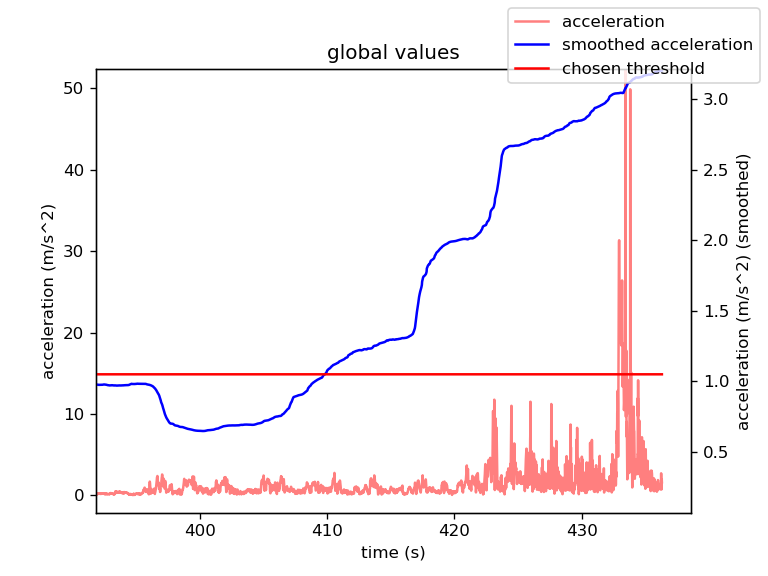
\includegraphics[width=5in]{fig4.png}
\captionof{figure}{Zoom sur la partie du graphe concernant la chute}
\end{center}
\section{Calcul du ratio de temps en mouvement}
\label{sec:org1c7c718}

\begin{minted}[]{python}
moving_time = time[absolute_smooth > thresh]

moving_ratio = len(moving_time) / len(time) 
print(f"{np.round(moving_ratio*100, 2)} %")
\end{minted}

\begin{quote}
=> 45.54 \%
\end{quote}

\textcolor{darkblue}{La première instruction crée un tableau ne contenant que les valeurs supérieures à notre seuil (thresh qui avait été défini grâce à interract). La longueur des tableaux time et moving\_time correspond au nombre de secondes qu'ils contiennent, la ligne suivante fait donc le rapport entre les deux et la dernière ligne affiche le résultat.}
\section{Conclusion}
\label{sec:org47b23fb}

\textcolor{darkblue}{Dans ce rapport, nous avons donc analysé les données mesurées avec phyphox lors de la dernière séance d'escalade. Nous avons tenté d'obtenir la vitesse sans succès du fait de potentiel problème matériel ou de calibrage sur l'accéléromètre, une autre cause potentielle est une erreur dans les calculs ou le traitement des données. Pour régler le problème, il faudrait donc soit changer d'accéléromètre, soit recalibrer l'accéléromètre soit changer sa méthode de calcul et d'analyse des données. Nous avons ensuite tenté de filtrer le bruit à l'aide d'une moyenne roulante pour pouvoir ensuite calculer le temps d'escalade et le temps de chutes, nous avons obtenue des valeurs irréalistes pour le temps de chute. Les causes et résolution potentielles sont les mêmes que pour la vitesse. Ne pouvant exploiter ni le temps d'escalade, ni le temps de chute, il n'a pas été possible de calculer à partir du rapport entre ces données et celles de la vitesse, elle-même inexploitable, la hauteur du mur ou de la chute. La dernière section correspondait au calcul eu ratio du temps de mouvement sur le temps total, mais dans la mesure où les données de temps pour la chute et l'escalade était irréaliste, le résultat de ce même calcul parait peu fiable.}
\end{document}
